\documentclass{tufte-handout}

\title{Propositional Probability II: A Propositional PPL\thanks{CS7470 Fall 2023: Foundations of Probabilistic Programming.}}


\newcommand{\varset}[0]{\mathcal{V}}

\author[]{Steven Holtzen\\s.holtzen@northeastern.edu}

%\date{28 March 2010} % without \date command, current date is supplied

%\geometry{showframe} % display margins for debugging page layout
\setcounter{secnumdepth}{1}

\usepackage{graphicx} % allow embedded images
  \setkeys{Gin}{width=\linewidth,totalheight=\textheight,keepaspectratio}
  \graphicspath{{graphics/}} % set of paths to search for images
\usepackage{amsmath,amssymb,amsthm}  % extended mathematics
\usepackage{booktabs} % book-quality tables
\usepackage{units}    % non-stacked fractions and better unit spacing
\usepackage{multicol} % multiple column layout facilities
\usepackage{lipsum}   % filler text
\usepackage{fancyvrb} % extended verbatim environments
  \fvset{fontsize=\normalsize}% default font size for fancy-verbatim environments
\usepackage{listings}
\usepackage{tikz}
\usepackage{mathpartir}
\usepackage{subcaption}
\usepackage{mdframed}
\usepackage{epigraph}
\usepackage{enumitem}
\usepackage{stmaryrd}

\usetikzlibrary{shapes.geometric}


\usepackage[ruled,linesnumbered]{algorithm2e}
\SetKwComment{Comment}{/* }{ */}
\newcommand{\indep}{\perp \!\!\! \perp}

\tikzset{
  treenode/.style = {shape=rectangle, rounded corners,
                     draw, align=center,
                     },
  root/.style     = {treenode, font=\Large, bottom color=red!30},
  env/.style      = {treenode, font=\ttfamily\normalsize},
  dummy/.style    = {circle,draw}
}

% tikz
\usetikzlibrary{patterns,calc,backgrounds}


% TIKZ
\tikzstyle{nnf}=[
  >=stealth,font=\small,auto,scale=0.7,every node/.style={scale=0.7}
]
\tikzstyle{extnode}=[
  draw,circle,inner sep=2pt,fill=white
]

\tikzstyle{leafnode}=[
  draw,fill=gray!20,inner sep=3.5pt
]
\tikzstyle{constnode}=[
  draw,fill=white,inner sep=3.5pt
]
\tikzstyle{label}=[
  fill=white,inner sep=2.5pt
]

\tikzstyle{acarrow}=[
    decoration={markings,mark=at position 1 with {\arrow[scale=0.6]{>}}},
    postaction={decorate},
    shorten >=0.4pt,
    >=latex,
    line width=0.1
]

\tikzstyle{bnarrow}=[
    decoration={markings,mark=at position 1 with {\arrow[scale=1.5]{>}}},
    postaction={decorate},
    shorten >=0.7pt,
    >=latex,
    line width=0.3
]
\tikzstyle{bayesnet}=[
  >=latex, thick, auto
]
\tikzstyle{bnnode}=[
  draw,ellipse,minimum size=7mm,inner sep=1pt,font=\small
]
\tikzstyle{cpt}=[
  font=\footnotesize
]

\tikzstyle{graph}=[
  >=stealth,font=\small,auto,scale=1,every node/.style={scale=1}
]
\tikzstyle{node}=[
  draw,circle,inner sep=3pt,fill=white
]

% BDDs

\tikzstyle{bdd}=[
  >=latex, thick, >=stealth, font=\small,auto,scale=0.9,every node/.style={scale=0.9}
]
\tikzstyle{bddnode}=[
  draw,circle,inner sep=0pt,fill=white,minimum size=5.5mm
]

\tikzstyle{bddtriangle}=[
  draw, regular polygon, regular polygon sides = 3,inner sep=1pt,fill=white,minimum size=5.5mm
]

\tikzstyle{highedge}=[
    line width=0.9
]
\tikzstyle{lowedge}=[
    line width=0.9,dotted
]
\tikzstyle{bddterminal}=[
  draw,fill=gray!20,inner sep=2.5pt, font=\small
]

\lstdefinestyle{compact}{
  \ttfamily\tiny
}


\usetikzlibrary{positioning}

\newtheorem{theorem}{Theorem}
\newtheorem{definition}{Definition}
\newtheorem{conjecture}{Conjecture}
\newtheorem{lemma}{Lemma}
\newtheorem{exercise}{Exercise}
\newtheorem{remark}{Remark}


\usepackage{xcolor}

\definecolor{codegreen}{rgb}{0,0.6,0}
\definecolor{codegray}{rgb}{0.5,0.5,0.5}
\definecolor{codepurple}{rgb}{0.58,0,0.82}
\definecolor{backcolour}{rgb}{0.95,0.95,0.92}

\lstdefinestyle{mystyle}{
    backgroundcolor=\color{backcolour},   
    commentstyle=\color{codegreen},
    keywordstyle=\color{magenta},
    numberstyle=\tiny\color{codegray},
    stringstyle=\color{codepurple},
    basicstyle=\ttfamily\footnotesize,
    breakatwhitespace=false,         
    breaklines=true,                 
    captionpos=b,                    
    keepspaces=true,                 
    numbers=left,                    
    numbersep=5pt,                  
    showspaces=false,                
    showstringspaces=false,
    showtabs=false,                  
    tabsize=2
}

\lstset{style=mystyle}

\newcommand{\defn}[1]{\textbf{#1}}
\newcommand{\dbracket}[1]{\left \llbracket {#1} \right \rrbracket}
\newcommand{\dist}[1]{\mathtt{Dist}(#1)}
\newcommand{\true}[0]{\texttt{true}}
\newcommand{\te}[0]{\texttt{e}}
\newcommand{\false}[0]{\texttt{false}}
\newcommand{\real}[0]{\mathbb{R}}
\newcommand{\rational}[0]{\mathbb{Q}}
\newcommand{\lebesgue}[0]{\mathbb{L}}
\newcommand{\eval}[0]{\mathrm{ev}}
\newcommand{\disc}[0]{\textsc{Disc}}
\newcommand{\borel}[0]{\mathcal{B}}
\newcommand{\ent}[0]{\mathbb{S}}
\newcommand{\prog}[0]{\texttt{p}}
\newcommand{\bool}[0]{\mathbb{B}}
\newcommand{\cont}[0]{\textsc{Cont}}
\newcommand{\prop}[0]{\textsc{Prop}}
\newcommand{\bdd}[0]{\textsc{Bdd}}
\newcommand{\robdd}[0]{\textsc{Robdd}}
\newcommand{\compiles}[0]{\rightsquigarrow}

\newcommand{\bddtriangle}[1]{
    \begin{tikzpicture}
    \node [bddtriangle] {#1};
    \end{tikzpicture}}
\newcommand{\bddtrue}[0]{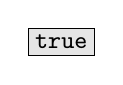
\begin{tikzpicture}
      \node [bddterminal] {$\true$};
    \end{tikzpicture}}
\newcommand{\bddfalse}[0]{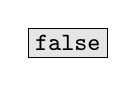
\begin{tikzpicture}
      \node [bddterminal] {$\false$};
    \end{tikzpicture}}


% Standardize command font styles and environments
\newcommand{\doccmd}[1]{\texttt{\textbackslash#1}}% command name -- adds backslash automatically
\newcommand{\docopt}[1]{\ensuremath{\langle}\textrm{\textit{#1}}\ensuremath{\rangle}}% optional command argument
\newcommand{\docarg}[1]{\textrm{\textit{#1}}}% (required) command argument
\newcommand{\docenv}[1]{\textsf{#1}}% environment name
\newcommand{\docpkg}[1]{\texttt{#1}}% package name
\newcommand{\doccls}[1]{\texttt{#1}}% document class name
\newcommand{\docclsopt}[1]{\texttt{#1}}% document class option name
\newenvironment{docspec}{\begin{quote}\noindent}{\end{quote}}% command specification environment



\begin{document}
\maketitle% this prints the handout title, author, and date

Now we are ready to ask: \emph{can we use
propositional logic as the basis for an effective probabilistic model}?
The first question is: what is our sample space? It's clear so far that a logical 
choice of sample space is the set of all possibly instances for a fixed set 
of Boolean formulae; this sample space will have size $2^n$, where $n$ is the number 
of propositional variables.
Now, if we want to efficiently evaluate queries over this sample space, we need
need two more components:
\begin{enumerate}
    \item A way to efficiently represent a probability distribution on the sample space;
    \item A way to efficiently represent queries over that sample space.
\end{enumerate}

% We will explore answers to these questions today.

Let's tackle (1) first. What is an alternative representation of a distribution 
that avoids the space-explosion we saw in the lookup-table representation? We 
will need to be more clever about how we represent probabilities. One useful
choice is to assume that all random variables are \emph{independent from each other}, 
and therefore we can concisely describe a joint distribution over all of them:

\begin{definition}[Fully factorized probabilistic model]
    Let $X_1, X_2, \cdots, X_n$ be jointly independent random variables (i.e.,
    for any pair $X_i, X_j$, it is the case that $X_i \indep X_j$). Then, a
    fully-factorized probabilistic model is a collection of $n$ probability
    lookup tables $\Pr(X_i)$, one for each $i$. The joint probability is computed 
    as $\Pr(X_1, X_2, \cdots, X_n) \triangleq \prod_i^n \Pr(X_i)$.
\end{definition}

Observe that a fully-factorized model only requires $O(\sum_i |X_i|)$ space,
which is significantly smaller than $|\Omega|$.\sidenote{The notation $|X|$
refers to the size of a random variable's co-domain.} This is a big improvement
over plain lookup tables, but it comes at a cost of expressivity: there are some
distributions that cannot be represented in a fully-factorized way.

\section{A Propositional PPL (\prop{})}
\marginnote{These are fresh semantics and there may be bugs! If you see any let 
me know.}
\begin{itemize}
  \item We will introduce a simple probabilistic programming language based on 
  propositional logic called \prop{}.
  \item The syntax of \prop{} has two parts: a query $\varphi$, written in 
  propositional logic, and a fully-factorized distribution $w$ on propositional 
  variables:
\end{itemize}
Syntax of \prop{}:
\begin{lstlisting}[mathescape=true]
$\varphi ::= x \mid \varphi \land \varphi \mid \varphi \lor \varphi \mid \neg \varphi \mid \true \mid \false$ 
$w ::= [x \mapsto \theta_x, y \mapsto \theta_y, \cdots]$
p ::= $(\varphi, w)$
\end{lstlisting}

Example \prop{} program:

\begin{lstlisting}[mathescape=true]
($x \lor y$, [$x \mapsto 0.1, y \mapsto 0.2$])
\end{lstlisting}

\begin{itemize}

  \item In order to interpret programs, we need to define a \defn{propositional
  universe}, which tells us which propositional variables the program is defined
  over. We denote this universe $\Gamma$, which is a finite set of propositional
  variables.

  \item A syntactic term in \prop{} is \defn{well-typed by universe $\Gamma$} if every
  propositional variable that is free in \prop{} can is in $\Gamma$. If a term
  is well-typed by $\Gamma$, we write $\Gamma \vdash \texttt{p}$. We can
  formalize this description of $\Gamma$ inductively on \prop{} programs. First,
  we describe whether or not a propositional term is well-typed, $\Gamma \vdash
  \varphi$:
  \begin{mathpar}
    \inferrule{}{\Gamma \vdash \true} \and \inferrule{}{\Gamma \vdash \false} \and
    \inferrule{x \in \Gamma}{\Gamma \vdash x} \\
    \inferrule{\Gamma \vdash \alpha \and \Gamma \vdash \beta}{\Gamma \vdash \alpha \land \beta}
  \end{mathpar}
  The rest of the propositional connectives proceed similarly.

  \item Similarly, we can type the $w$ terms:
   \begin{mathpar}
    \inferrule{x \in \Gamma \and \Gamma \vdash r}{\Gamma \vdash [x \mapsto \theta, r]} \and 
    \inferrule{}{\Gamma \vdash []}
  \end{mathpar}
 
  \item Finally, we can type programs:
  \begin{mathpar}
    \inferrule{\Gamma \vdash \varphi \and \Gamma \vdash w}{\Gamma \vdash (\varphi, w)}
  \end{mathpar}

  \item We can interpret a propositional universe $\Gamma$ as the set of all
  propositional instances that can be formed from variables in $\Gamma$; we 
  write this set as $\dbracket{\Gamma}$.
  
\end{itemize}

\subsection{Denotational semantics}
\begin{itemize}
  \item Denotational semantics of \prop{}: we want to associate every well-typed
  program in \prop{} with the probability that $\varphi$ holds according to the
  fully-factorized distribution described by $w$


  \item \defn{Goal}: Define a map $\dbracket{\Gamma \vdash \texttt{p}} : [0,1]$ that maps well-typed terms from 
  \prop{} to real values. \marginnote{For more on the history and context of different 
  styles of semantics, see \citet[Chapter 3]{pierce2002types}}
  \item We will need semantics for $\varphi$ and the map $m$ in order to
  interpret \texttt{p}. 
  They have the following types:
  \begin{itemize}
    \item $\dbracket{\Gamma \vdash \varphi}$ maps propositional formulae to the
    set of all instances that model them over universe drawn from $\Gamma$:
    \begin{align}
     \dbracket{\Gamma \vdash \varphi} &\triangleq \{I \in \dbracket{\Gamma} \mid I \models \varphi \}
    \end{align}
    \item $\dbracket{\Gamma \vdash w} : \Gamma \rightarrow \bool \rightarrow [0, 1]$ produces a
    map from assignments to propositional variables to real values:
  \end{itemize}
  \begin{align}
    \dbracket{\Gamma \vdash [x_1 \mapsto \theta_1, \dots, x_n \mapsto \theta_n]}(x_i)(\true) &\triangleq \theta_i\\
    \dbracket{\Gamma \vdash [x_i \mapsto \theta_1, \dots, x_n \mapsto \theta_n]}(x_i)(\false) &\triangleq 1-\theta_i
  \end{align}
  We need to assume a propositional universe so that these equations are well-defined.
  Assume that all instances are defined on all free variables in $\texttt{p}$.
  \item For notational convenience we define the probability of an instance $\dbracket{\Gamma \vdash w}(I)$
  as the product of probabilities of each variable in the instance. For
  instance,
  \begin{align*}
    \dbracket{(x \mapsto 0.1, y \mapsto 0.3)}(x, \overline{y}) = 
    0.1 * 0.7.
  \end{align*}
  Formally, we will write:
  \begin{align}
    \dbracket{\Gamma \vdash w}(I) = \prod_{[x_i \mapsto v] \in I}\dbracket{w}(x_i)(v)
  \end{align}
  \item Now we are ready to interpret \prop{} programs as the sum of the probabilities 
  of each model:
  \begin{align}
    \dbracket{\Gamma \vdash (\varphi, w)} \triangleq \sum_{I \in \dbracket{\Gamma \vdash \varphi}} \dbracket{\Gamma \vdash w}(I).
  \end{align}
\end{itemize}

\begin{itemize}
  \item Is this a \emph{useful} PPL? What kinds of programs 
  can we write in it? Exercise: write a \prop{} program that 
  computes the probability that a dice roll is even.
\end{itemize}

\section{Big-step semantics}
\begin{itemize}
  \item Our denotational model does not tell us how to efficiently compute probabilities
  \item \textbf{Goal}: given a \prop{} program, \emph{efficiently evaluate it}

    \textbf{Running example}: The simple \prop{} program:
\begin{lstlisting}[mathescape=true]
($x \lor y$, $[x \mapsto 0.1, y \mapsto 0.3]$)
\end{lstlisting}

    \item Worst-case hardness: computing $\Pr(\varphi_{ex})$ is NP-hard for 
    arbitrary formulae.

    We will show this by reduction to the \defn{SAT problem}: the problem of
    determining whether or not a formula has a model.

    Reduction: Let $\varphi$ be a formula. Assign a probability of 0.5 to 
    every assignment of variables. Then, $\varphi$ has a model if and 
    only if $\Pr(\varphi) > 0$.
    
    \item In fact, computing $\Pr(\varphi_{ex})$ is \#P-hard. 
    \#P is the class of problems that are polytime reducible to counting 
    the number of solutions to an arbitrary Boolean formula.
    See \citet[Chapter
    6]{goldreich2008computational} for more discussion on this complexity class, 
    as well as \citet{roth1996hardness}.
\end{itemize}

\subsection{Evaluating queries via search}
\begin{itemize}
  \item Need to avoid worst-case exponential behavior.
  \item \emph{Idea}: We want to \emph{search} through the space of models of
  the formula to potentially avoid exploring all possible worlds. Aim for better 
  average-case/common-case behavior than the naive table enumeration.
    
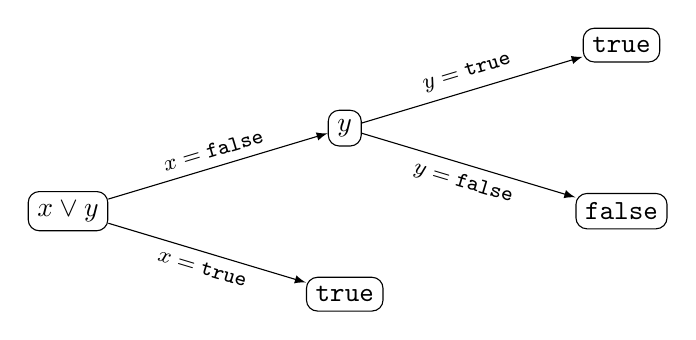
\begin{tikzpicture}
    [
      grow                    = right,
      sibling distance        = 6em,
      level distance          = 10em,
      edge from parent/.style = {draw, -latex},
      every node/.style       = {font=\footnotesize},
      sloped
    ]
    \node [env] {$x \lor y$}
      child { node [env] {$\true$}
        edge from parent node [below] {$x = \true$} }
      child { node [env] {$y$}
        child { node [env] {$\false$}
          edge from parent node [below] {$y = \false$} }
        child { node [env] {$\true$}
                edge from parent node [above, align=center]
                  {$y = \true$}}
                edge from parent node [above] {$x = \false$} };
  \end{tikzpicture}

    \item We will describe a relation $(\pi, \texttt{p}) \Downarrow^e \real$:
    \begin{itemize}[noitemsep]
        \item $\pi$ is an ordered list of propositional variables. We denote 
        list concatenation as $x::\pi$. 
        \item \texttt{p} is a \prop{} program
        \item The result $\mathbb{R}$ will be equal to $\dbracket{\texttt{p}}$
    \end{itemize}

    \item Define $\varphi[x \mapsto v]$ as the substitution where we replace all
    instances of $x$ with the value $v \in \{\true, \false\}$ in $\varphi$, and
    ``simplify'' $\varphi$ by evaluating connectives until either (1) there are no more 
    $\true$ or $\false$ constants, or (2) the formula is equal to $\true$ or $\false$. 
    \\
    Example: $(x \lor y)[x \mapsto \true] = y$.

    \item 
    Now, let's describe our procedure for searching to solve our
    inference problem. 
    We will define $\Downarrow^e$ inductively. The base-cases will be 
    formulas without any free variables: 
    \begin{mathpar}
    \inferrule[\textsc{(True)}]{}{(\pi, (\true, w)) \Downarrow^e 1}
    \and
    \inferrule[\textsc{(False)}]{}{(\pi, (\false, w)) \Downarrow^e 0}
    \end{mathpar}

    \item Then, the inductive step:
  \begin{mathpar}
    \inferrule[\textsc{(Split)}]{(\pi, (\varphi[x \mapsto \true], w)) \Downarrow^e v_1 \and 
    (\pi, (\varphi[x \mapsto \false], w)) \Downarrow v_2
    }{(x :: \pi, (\varphi, w)) \Downarrow^e w(x)v_1 + w(\overline{x}) v_2} \\
\end{mathpar}

  Here we are being a bit loose with the weight function $w$; we can give an evaluation 
  semantics for $w$ as well, but assume for now that we can look up the weight of $x$ and 
  $\overline{x}$.


  \item Example derivation tree for our running example for the order $\pi = [x, y]$ 
  and our program ($x \lor y$, $[x \mapsto 0.1, y \mapsto 0.3]$)

  % \begin{mathpar}
  %     \inferrule
  %     {\inferrule{\inferrule{([], (\true, w) \Downarrow^e 1)} \and ([], (\false, w) \Downarrow^e 0)}}{(y::[], y) \Downarrow } }
  %     {(x::[y], (x \lor y, w)) \Downarrow }
  % \end{mathpar}

  \item The \defn{cost} of evaluating a formula $\varphi$ for order $\pi$ under
  these semantics is equal to the total number of derivations in the derivation
  tree.
\end{itemize}

\begin{theorem}
  Let \texttt{p} be \prop{} program and $\pi$ be an ordering on all 
  variables in \texttt{p}, and let $\Gamma \vdash \texttt{p}$. 
  If $(\pi, \texttt{p}) \Downarrow v$, then
  $\dbracket{\Gamma \vdash \texttt{p}} = v$.
\end{theorem}

% To prove this theorem we will need the following \emph{extensionality property},
% gives some conditions on which two propositional terms that are both well-typed 
% always have identical denotation:
% \begin{lemma}[Extensionality]
%   If $\Gamma_1 \subseteq \Gamma_2$ and $\Gamma_1 \vdash (\varphi, w)$, then
%   $\dbracket{\Gamma_1 \vdash (\varphi, w)} = \dbracket{\Gamma_2 \vdash (\varphi, w)}$.
% \end{lemma}
% \begin{proof}
%   The proof is by induction on $|\Gamma_2|$.
%   \begin{itemize}
%     \item Base case: Assume $|\Gamma_1| = |\Gamma_2|$. Then
%     by definition $\Gamma_1 = \Gamma_2$, so the claim follows.
%     \item Induction: Assume $\Gamma_1 \subseteq \Gamma$
%     and that $\dbracket{\Gamma \vdash (\varphi,
%     w)} = \dbracket{\Gamma_1 \vdash (\varphi, w)}$. Then, show that
%     $\dbracket{\Gamma \cup \{x\} \vdash (\varphi, w)} = \dbracket{\Gamma
%     \vdash (\varphi, w)}$. 

    
%     We proceed:
%     \begin{align*}
%       \dbracket{\Gamma \cup \{x\} \vdash (\varphi, w)} &= 
%       \sum_{I \in \dbracket{\Gamma \cup \{x\} \models \varphi}} \dbracket{\Gamma \cup \{x\} \vdash w}(I)\\
%       &= \sum_{I \cup [x \mapsto \true] \in \dbracket{\Gamma \vdash \varphi}} \dbracket{\Gamma \vdash w}(I)
%     \end{align*}
%     To use our inductive hypothesis we need to break $\dbracket{\Gamma \vdash \varphi}$ up 
%     into smaller pieces. We can do this by observe that
%   \end{itemize}
% \end{proof}

% Now we can prove the main theorem:

\begin{proof}[Proof sketch]
  We will show this by structural induction on \texttt{p}. 
  The base cases are straightforward: If $\texttt{p} = (\true, w)$, then 
  $(\pi, (\true, w)) \Downarrow^e 1$. By definition, $\dbracket{\Gamma \vdash (\true, w)} = \sum_{I \in \dbracket{\Gamma \vdash \true}} w(I) = 1$; 
  similar for the false case.

  Induction hypothesis (IH): Let $(x::\pi, (\varphi[x \mapsto \true], w))
  \Downarrow^e v_1$ and $(x::\pi, (\varphi[x \mapsto \false], w)) \Downarrow^e
  v_2$, and $(\pi, (\varphi, w)) \Downarrow^e v$. Assume by induction that $v_1
  = \dbracket{\Gamma \vdash (\varphi[x \mapsto \false], w)}$ and $v_2 =
  \dbracket{\Gamma \vdash (\varphi [x \mapsto \true], w)}$. 
  
  We are done if we can show that
$\dbracket{\Gamma \vdash (\varphi, w)} =
\dbracket{w}(x)(\true)\dbracket{\Gamma \vdash (\varphi[x \mapsto \true], w)} +
\dbracket{w}(x)(\false)\dbracket{\Gamma \vdash (\varphi[x \mapsto \false], w)}$.

To make progress we need to apply \emph{Shannon expansion}: it is always the case that 
$\dbracket{\Gamma \vdash (\varphi, w)} = \dbracket{\Gamma \vdash (\varphi \land x, w)} + 
\dbracket{\Gamma \vdash (\varphi \land \neg x, w)}$.\marginnote{The proof of Shannon expansion 
is a good exercise, and relies on splitting up the models of $\varphi$ into 2 sets.}
Then, observe that $\dbracket{\Gamma \vdash (\varphi \land x), w} = w(x)(\true)
\dbracket{\Gamma \vdash (\varphi[x \mapsto \true], w)}$ (this fact is not as straightforward
to show as Shannon expansion, and proving it rigorously relies on a 
full inductive definition of substitution, so we elide step for the time being). 

  % Then, 
  % \begin{align*}
  %   \dbracket{\Gamma \vdash (\varphi, w)} &= \sum_{I \in \dbracket{\Gamma \vdash \varphi}} \dbracket{\Gamma \vdash w}(I)
    % &= \sum_{\{I \in \dbracket{\varphi \land x}\}} w(I) + 
    % \sum_{\{I \in \dbracket{\varphi \land \overline{x}}\}} w(I) \\ 
  % \end{align*}



% Then, if we can show that $\dbracket{\varphi \land x, w} =
% w(x)\dbracket{\varphi[x \mapsto \true], w} =w(x)v_1$ (and analogously for the false
% case), then we are done. One way to show this is by induction on the structure of 
% terms in propositional logic (we could also make a model-based argument; it's a good exercise 
% to think about what that proof would look like). Here is the structural induction argument for 
% practice.

% \begin{lemma}
%   $\dbracket{\Gamma \vdash (\varphi \land x, w)} = w(x)\dbracket{\Gamma \vdash (\varphi[x \mapsto \true], w)}$.
% \end{lemma}
% Base cases: 
% \marginnote{This argument is made more cumbersome 
%   by the fact that the size of our propositional universe is implicit in our definition of $\dbracket{\cdot}$.}
% \begin{itemize}
%   \item $\varphi = \true$. Then, 
%   \begin{align*}
%     \dbracket{ \true \land x, w} = \dbracket{x, w} =^{\star} w(x) = w(x)\dbracket{\true[x \mapsto \true], w}
%   \end{align*}
%   Showing the equality marked $\star$ is the crucial step. To show we can use another 
%   tiny inductive argument on the size of our propositional universe $N$ (i.e., the 
%   number of propositional variables). 
%   \begin{itemize}
%     \item Assume $N=1$. Then, $\dbracket{x, w} = $
%     \item Inductive hypothesis: 
%   \end{itemize}
  % \begin{align*}
  %   \dbracket{x} = \sum_{I \in \dbracket{x}} w(I) = \sum_{I \in \dbracket{x}} \prod_{ \ell \in I} w(\ell), 
  % \end{align*}
  % where $\ell$ is an individual variable assignment in the instance $I$, and
  % $w(\ell)$ is the probability given that that assignment by $w$. Then, we can continue the above 
  % by reordering:
  % \begin{align*}
  %   \sum_{I \in \dbracket{x}} \prod_{ \ell \in I} w(\ell) &= 
  %   \sum_{I \in \dbracket{x}} \prod_{\ell \in I} w(\ell)
  % \end{align*}
%   \item $\varphi = \false$. Then, $\dbracket{ \false \land x} = \dbracket{\false} = 0 = w(x)\dbracket{\false[x \mapsto \true]}$.
%   \item $\varphi = x$. Then, $\dbracket{ x \land x} = \dbracket{x} = w(x) = w(x)\dbracket{x[x \mapsto \true]}$\\
%   \item $\varphi = y$. Then, $\dbracket{ x \land y} = w(x)w(y) = w(x)\dbracket{x \land y[x \mapsto \true]}$
% \end{itemize}

% Now for the inductive cases. 



% Example: consider the formula $x \lor y$. Then: \begin{align*} \dbracket{(x \lor
% y, w)} = \underbrace{w(xy) + w(x\overline{y})}_{(A)} +
% \underbrace{w(\overline{x}y)}_{(B)} \end{align*}

% Since $v = w(x) v_1 + w(\overline{x})v_2 = w(x) \dbracket{(\varphi[x \mapsto \true], w)} + 
% w(\overline{x}\dbracket{(\varphi[x \mapsto \false], w)})$ by IH, we are done if we can show that 
% $(A) = w(x) \dbracket{(\varphi[x \mapsto \true], w)}$ and $(B) =
% w(\overline{x})\dbracket{(\varphi[x \mapsto \false], w)}$.

% To show this observe that after substituting, $x$ is no longer in $\varphi[x \mapsto v]$. 
% Example:
% \begin{align*}
%   \dbracket{(x \lor y)[x \mapsto \false]} &= \dbracket{y}\\
%   &= w(xy) + w(\overline{x}y) \\
%   &= w(x)w(y) + w(\overline{x})w(y)\\ 
%   &= w(y)
% \end{align*}
% As the above calculuation shows, due to the factorization of $w$, we can prove
% that:
% \begin{align*}
%   \dbracket{(\varphi[x \mapsto \true], w)} = w(x)\dbracket{(\varphi, w)}.
% \end{align*}

\end{proof}



\begin{itemize}
  \item What is the cost of enumerating the formula $x \lor y \lor z \lor w$ with these 
  semantics? It will be linear-time for any order; a big improvement over the 
  exhaustive enumeration!

  \item However, what about a formula like $(a \land b) \lor (c \land d)$? We will see how to 
  handle this case next time.
\end{itemize}

% \section{Memoization}

% \begin{itemize}
%   \item This process is sometimes also called \emph{variable elimination}
%   \item Add a context to the reduction relation $\rho: \varphi \rightarrow [0,
%   1]$ that maps formulae to their probability of being true
%   \item Relation now has the shape:
%   \begin{align*}
%     (\pi, \rho, \texttt{p}) \Downarrow^m (\real, \rho')
%   \end{align*}
% \end{itemize}




% In the context of propositional logic, there is a natural notion of a
% fully-factorized model. Let $\Omega$ be the collection of $n$-element instances.
% Then, each propositional variable corresponds to a projection out of that sample
% space. Let's call this the \defn{fully factorized propositional distribution}: each 
% variable in the theory will be associated with an independent probability of 
% being $\true$ or $\false$. For example, we may have to propositional variables $x$ and 
% $y$; the fully factorized distribution could be given by two independent lookup tables:
% \begin{align}
%     [x \mapsto 0.1, \overline{x} \mapsto 0.9], \quad [y \mapsto 0.2, \overline{y} \mapsto 0.8].
%     \label{eq:indepdist}
% \end{align}
% Then, the joint probability $\Pr(x, \overline{y})$ is $0.1 \times 0.8$.

% \newthought{Now we return to an earlier question}: how do we efficiently represent 
% events in the propositional setting? Events are a subset of the sample space. 
% The sample space in propositional probability is the set of all instances. Then, 
% we can represent events by \emph{propositional formulae}:
% \begin{align}
%     \Pr(\varphi) \triangleq \sum_{I \models \varphi} \Pr(\varphi).
% \end{align}
% For instance, for the fully-factorized 
% distribution in Eq.~\ref{eq:indepdist}, we can compute the probability of a 
% propositional sentence $x \lor y$ by summing the probability mass over each 
% instance that models this formula:
% \begin{align}
%     \Pr(x \lor y) = \Pr([x, y]) + \Pr([x, \overline{y}]) + \Pr(\overline{x}, y).
% \end{align}

% This is implemented by the following algorithm:

% \begin{algorithm}
%     \caption{QueryPropositionalEvent$_1$($\Pr, \varphi)$}
%     \KwData{A fully-factorized distribution $\Pr$; a propositional formula $\varphi$}
%     \KwResult{The probability of the event $\Pr(\varphi)$}
%     $a \leftarrow 0$\;
%     \For{each $I \in \Omega$}{
%         \lIf{$I \models \varphi$}{$a \leftarrow a + \Pr(\omega)$}
%     }
%     \Return{a}
%     \label{alg:enum}
% \end{algorithm}


% Unfortunately, QueryPropositionalEvent is \emph{still linear} in the size of
% $|\Omega|$ due to the outer loop on Lines 2--4.  In all cases, regardless of the
% structure of $\varphi$, we have to consider all all the instances, which will
% not scale. 

% \subsection{Efficiently evaluating queries via search}
% How do we avoid scaling in $|\Omega|$ during querying? 
% In other words: is it possible to design a scalable automated reasoning strategy 
% for our tiny probabilistic programming language that we've made so far, with fully-factorized 
% propositional distributions and queries given as propositional formulae?
% In the worst case, it
% may not be possible to avoid considering all possible instances, but we can 
% try to avoid this worst-case explosion by delicately \emph{exploiting the problem 
% structure}: in particular, we want to simultaneously exploit the fully-factorized 
% structure of the distribution along with the fact that all events are written 
% as propositional formulae.

% One approach is to \emph{exploit the structure of models of the query
% $\varphi$}: sometimes, a query may only have a single model, or perhaps most
% instances are models. In these cases, we waste a lot of effort enumerating all
% models; it is much more efficient to \emph{search} for the few satisfying instances.

% For example, consider the formula $x \lor y$. We can recursively decompose this
% formula by branching on assignments to propositional variables:

% \begin{tikzpicture}
%     [
%       grow                    = right,
%       sibling distance        = 6em,
%       level distance          = 10em,
%       edge from parent/.style = {draw, -latex},
%       every node/.style       = {font=\footnotesize},
%       sloped
%     ]
%     \node [env] {$x \lor y$}
%       child { node [env] {$\true$}
%         edge from parent node [below] {$x = \true$} }
%       child { node [env] {$y$}
%         child { node [env] {$\false$}
%           edge from parent node [below] {$y = \false$} }
%         child { node [env] {$\true$}
%                 edge from parent node [above, align=center]
%                   {$y = \true$}}
%                 edge from parent node [above] {$x = \false$} };
%   \end{tikzpicture}

% The root of this binary tree is the original formula $x \lor y$. Each branch 
% assigns a propositional variable to a Boolean value. The children are 
% the resulting formula evaluated on the \emph{partial instance} given by the 
% path up until that point: for instance, if we assign $x = \false$, we are left 
% with the formula $\false \lor y = y$. Leaves of the tree denote whether or not a 
% particular assignment is a model.\sidenote{% source: https://tex.stackexchange.com/questions/188183/latex-under-construction-in-work-or-work-in-progress-symbols
\scalebox{0.5}[0.5]{
    (under construction)

\begin{tikzpicture}[limb/.style={line cap=round,line width=1.5mm,line join=bevel}]
\draw[line width=2mm,rounded corners,fill=yellow] (-2,0) -- (0,-2) -- (2,0) -- (0,2) -- cycle;
\fill (1.5mm,7mm) circle (1.5mm);
\fill(0,-7.5mm) -- ++(10mm,0mm) -- ++(120:2mm)--++(100:1mm)--++(150:2mm) arc (70:170:2.5mm and 1mm);
\draw[limb] (-7.5mm,-6.5mm)--++(70:4mm)--++(85:4mm) coordinate(a)--++(-45:5mm)--(-2.5mm,-6.5mm);
\fill[rotate around={45:(a)}] ([shift={(-0.5mm,0.55mm)}]a) --++(0mm,-3mm)--++
        (7mm,-0.5mm)coordinate(b)--++(0mm,4mm)coordinate(c)--cycle;
\draw[limb] ([shift={(-0.6mm,-0.4mm)}]b) --++(-120:5mm) ([shift={(-0.5mm,-0.5mm)}]c) --++
        (-3mm,0mm)--++(-100:3mm)coordinate (d);
\draw[ultra thick] (d) -- ++(-45:1.25cm);
\end{tikzpicture}
}}

% % this can be described using big-step!
% \begin{algorithm}
%     \caption{PrEvent($\Pr, \varphi$)}
%     \KwData{A fully-factorized distribution $\Pr$; a propositional formula $\varphi$; a decision order $\sigma$.}
%     \KwResult{The probability $\Pr(\varphi)$.}
%     \lIf{$\varphi = \true$}{\Return 1}
%     \lIf{$\varphi = \false$}{\Return 0}
%     $v \leftarrow head(\sigma)$\;
%     $\sigma' \leftarrow tail(\sigma)$\;
%     $ \varphi_v \leftarrow $ fix $v = \true$ in $\varphi$\;
%     $ \varphi_{\overline{v}} \leftarrow $ fix $v = \false$ in $\varphi$\;
%     \Return{$\Pr(v) \times $PrEvent$(\Pr, \varphi_v) + \Pr(\overline{v}) \times $PrEvent$(\Pr, \varphi_{\overline{v}})$}
%     \label{alg:rec}
% \end{algorithm}

% You should convince yourself that the above algorithm is correct by trying it on a few examples. 
% It is a good exercise to prove it correct inductively.
% What is the runtime of Algorithm~\ref{alg:rec}? In the worst-case, it is still $|\Omega|$. But, 
% sometimes -- depending on the structure of $\varphi$ -- it can do better by terminating the 
% recursion earlier in a base-case on Lines 1 and 2, rather than exhaustively exploring all 
% instances like Algorithm~\ref{alg:enum}.



% % Now, suppose we are given a probability measure $\Pr$ on instances. Now we want
% % to ask: \emph{what is the probability that a particular sentence $\varphi$ is
% % true for this world?} A subset of $\Omega$ is called an \defn{event}, and the 
% % probability of this particular event can be computed as the total probability of
% % all models of $\varphi$:
% % \begin{align}
% %     \Pr(\varphi) \triangleq \sum_{I \models \varphi} \Pr(I).
% %     \label{eq:pr2}
% % \end{align}
% % Note that above we overloaded the notation used for $\Pr$ to now act 
% % on events; this is common practice.
% % As an example, using the probability measure given in Table~\ref{tbl:simple}, we
% % can compute:
% % \begin{align}
% % \Pr(x \lor y) = \Pr([x, y]) + \Pr([x, \overline{y}]) + \Pr(\overline{x}, y) = 0.6.
% % \end{align}

% % \subsection{A propositional probabilistic programming language}
% % Tables like Table~\ref{tbl:simple} are a very inconvenient way to describe a
% % probability distribution. They are exponential in size, making them infeasible 
% % to write down for a large set of propositional variables, and they convey no useful 
% % structure to the user. In short, tables aren't a very useful probabilistic 
% % programming language.

% % It is much more convenient and usable 

% \begin{exercise}[$\star$]
%     Assume the following fully-factorized distribution on propositional variables:
%     \begin{align*}
%         [x \mapsto 0.1, \overline{x} \mapsto 0.9],\quad [y \mapsto 0.3, \overline{y} \mapsto 0.7].
%     \end{align*}
%     Use an exhaustive search tree to compute $\Pr(x \Leftrightarrow y)$.
% \end{exercise}
% \begin{exercise}[$\star\star$]
%     Prove Algorithm~\ref{alg:rec} correct.
% \end{exercise}


\bibliographystyle{plainnat}
\bibliography{../bib}

\end{document}